\subsection{AI-based data selection}

Traditionally, online data selection is performed using fixed topological cuts such as an energy deposit threshold in a calorimeter or the minimum transverse momentum of a track. Online data selection can benefit from the introduction of ML techniques typically used in offline data selection. It is advantageous to introduce these techniques at this stage to keep events that would be rejected by conventional methods and thereby increasing the overall physics output of a detector. This approach can also simultaneously reject events that have a level of noise that would render a physics analysis of this event impractical.

The consortium is constructing a system where these selection techniques can be realised directly in hardware and will initially be deployed at sPHENIX which will double as a test system for an EIC detector. This project involves two symbiotic AI systems; one to identify collisions containing heavy flavor decays through their unique topology and another to determine the beamspot for the detector during operation. The latter system then feeds back to the data selection system to improve the physics efficiency.


%There are several features of these decays which separate them from background such as tracks which do not point to the collision vertex, tracks which meet at a point away from the collision vertex (characteristic of the secondary vertex) and an overall increase in the number of tracks. It is possible that not all signatures of these decays are present in each signal candidate and so conventional selections tend to have a large number of background candidates by having sufficiently loose selections to overcome this. This situation is also worsened by the relatively small cross-sections for heavy flavor production compared to minimum bias collisions, there are approximately 50 background candidate for each $c\bar{c}$ pair produced~\cite{jackson2016measurement, aaij2013prompt}. Using AI to select these decays over conventional methods has the ability to drastically improve the signal-to-background ratio for several physics channels and, in a test case using simulated $D^0\rightarrow K^-\pi^+$ decays\footnote{charge-conjugation is implied} and background collisions, it was found that an untuned machine learning algorithm was able to increase the background rejection from 57.4$\,\pm\,$4.2$\%$ to 73.3$\,\pm\,$3.7$\%$ for comparable signal efficiencies (81.2$\,\pm\,$3.5$\%$ for the conventional method and 79.3$\,\pm\,$3.6$\%$ for the AI-based data selection). This test example was simulated using the sPHENIX detector which shares many similarities with the ECCE detector and it is expected that the background rejection can be improved with careful tuning of algorithms.

In the system, the accept decisions would be handled by a separate FELIX system which aggregates information from several subdetectors but it should be noted that the choice of technology could evolve along with general hardware developments in the next decade. The FELIX has 48 bi-directional links allowing for data from multiple systems to be passed to a single FELIX board. The machine learning algorithm will then be loaded onto the FPGA which will be capable of basic tracking (using tracklets from the vertex, sagitta and FST detectors) to make decisions that can be fed back to the initial DAQ or global data selection system to signal processing should continue. This should be achieved within 6$\,\mu$s\footnote{This requirement is determined by the shaping time of sPHENIX's vertex detector and could differ for ECCE}. The sPHENIX-based system will be restricted to using information from the trackers. Heavy flavor decays can also leave significant deposits in the calorimetry system but this is limited to 15\,kHz at sPHENIX. If this bottleneck can be remedied for ECCE, the selection system can be improved further. %Block diagrams of the FELIX board when used as a data selection system with the relevant data paths are given in Figure~\ref{fig:felix-ai}.

%\begin{figure}[hbt!]
%	\begin{center}
%		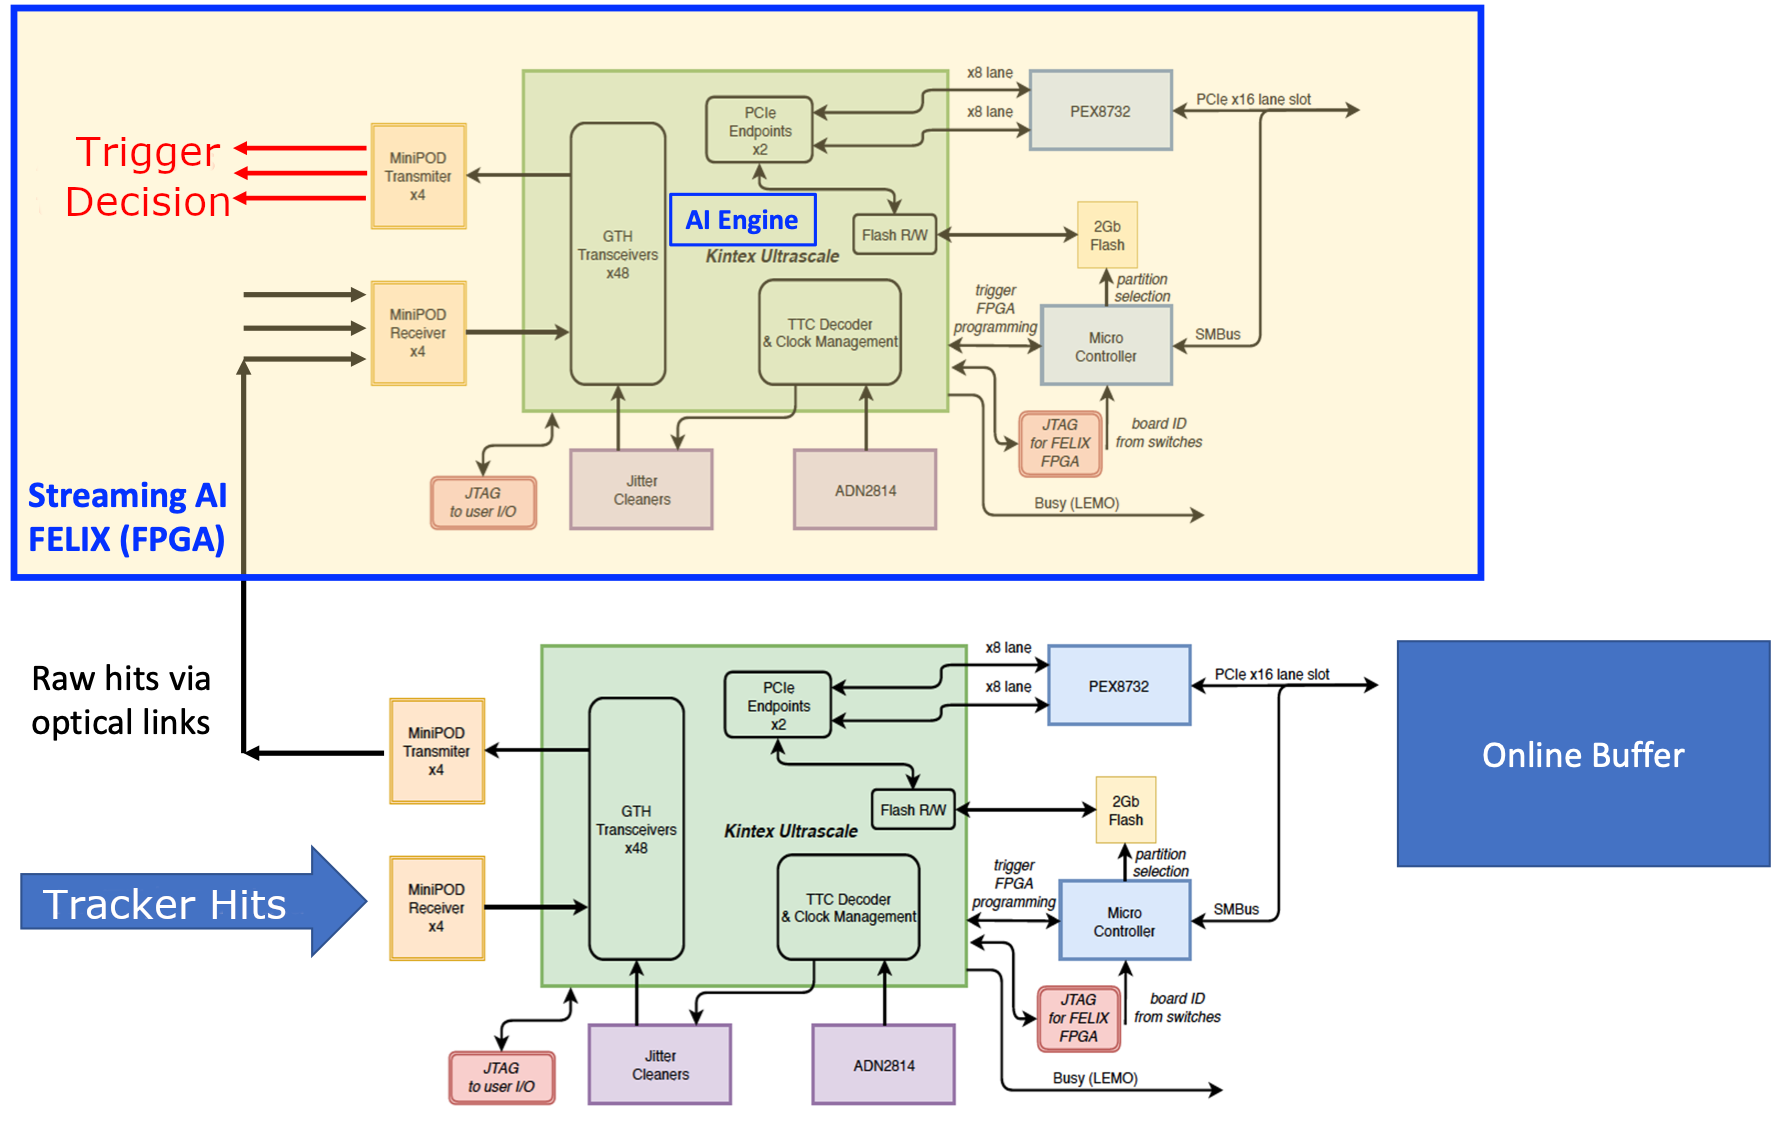
\includegraphics[width=0.8\textwidth]{figs/FELIX-AI}
%		
%		\caption[FELIX data selection System]{Block diagram of two FELIX boards when used as in the proposed smart data selection system. The FELIX on the bottom represents the conventional DAQ system that aggregates from subsections of the tracking system. There can be many of these systems. The top FELIX acts as the selection system, taking data from multiple systems and gives a single decision for each collision passed to it. The system combines the data and the Kintex Ultrascale contains GNNs capable of fast tracking and data selection.}\label{fig:felix-ai}
%	\end{center}
%\end{figure}

Studies are ongoing, comparing the outputs of algorithms trained using Convolution Neural Networks (CNNs) and Graph Neural Networks (GNN). For many applications, GNNs often represent a more robust ML algorithm than CNN due to using additional information from the edges of the graph as well as the node information used by a traditional CNN. This makes them more applicable to sparse data such as tracking and data selection where the overall occupancy of the detector system is low.

It is important to note that the beam conditions can change with time, this can be both during a run and on a longer scale. Thus it is imperative that, as well as developing a selection algorithm, we develop a feedback system that is capable of monitoring the beam conditions in real time and adapting the input parameters to this. For example, the position of the collision point directly impacts the measurement of the track displacement. If this moves, it will alter the signal and background efficiencies in opposite directions. This monitoring will be achieved using GPUs which will feedback to the selection system. GPUs typically perform well using CNNs which motivates the study of various machine learning methods to find the optimal set of algorithms to use for each stage of the selection and monitoring. Other important features that can appear in a detector, impacting this system and hence must be monitored are the appearance of noisy channels (or pixels) and displacement of parts of the detector, such as through thermal expansion or vibrations. It has been demonstrated that algorithms can run fast enough on GPUs to achieve this form of monitoring~\cite{gpu2021}.


%The project was approved in August 2021 and development of the algorithm is underway using simulated signal and background collisions. The algorithm will be translated for loading onto the FPGA using hls4ml~\cite{fahim2021hls4ml} and testbenches have been set up using 2 Xilinx development boards; a KC705 and VC709, the latter of which shares the same FPGA as the FELIX board. The KC705 will read simulated hits, in the same data format as the real detector, and send it to the VC709 via optical links and thus the KC705 emulates the DAQ and the VC709 emulates the selection system. The hls4ml package has already demonstrated the ability to translate ML algorithms to high level synthesis language which can be transferred to an FPGA as a bitstream and the stages required are shown in Figure~\ref{fig:hls4ml}. It has also been shown that the KC705 can receive data from host-to-client using Direct Memory Access (DMA). This project has been funded for two fiscal years and will use sPHENIX as a proof-of-principle. sPHENIX will cease operations before ECCE data taking and thus a smart data selection system is a realistic prospect for ECCE.


%\begin{figure}[hbt!]
%   \begin{center}
 %       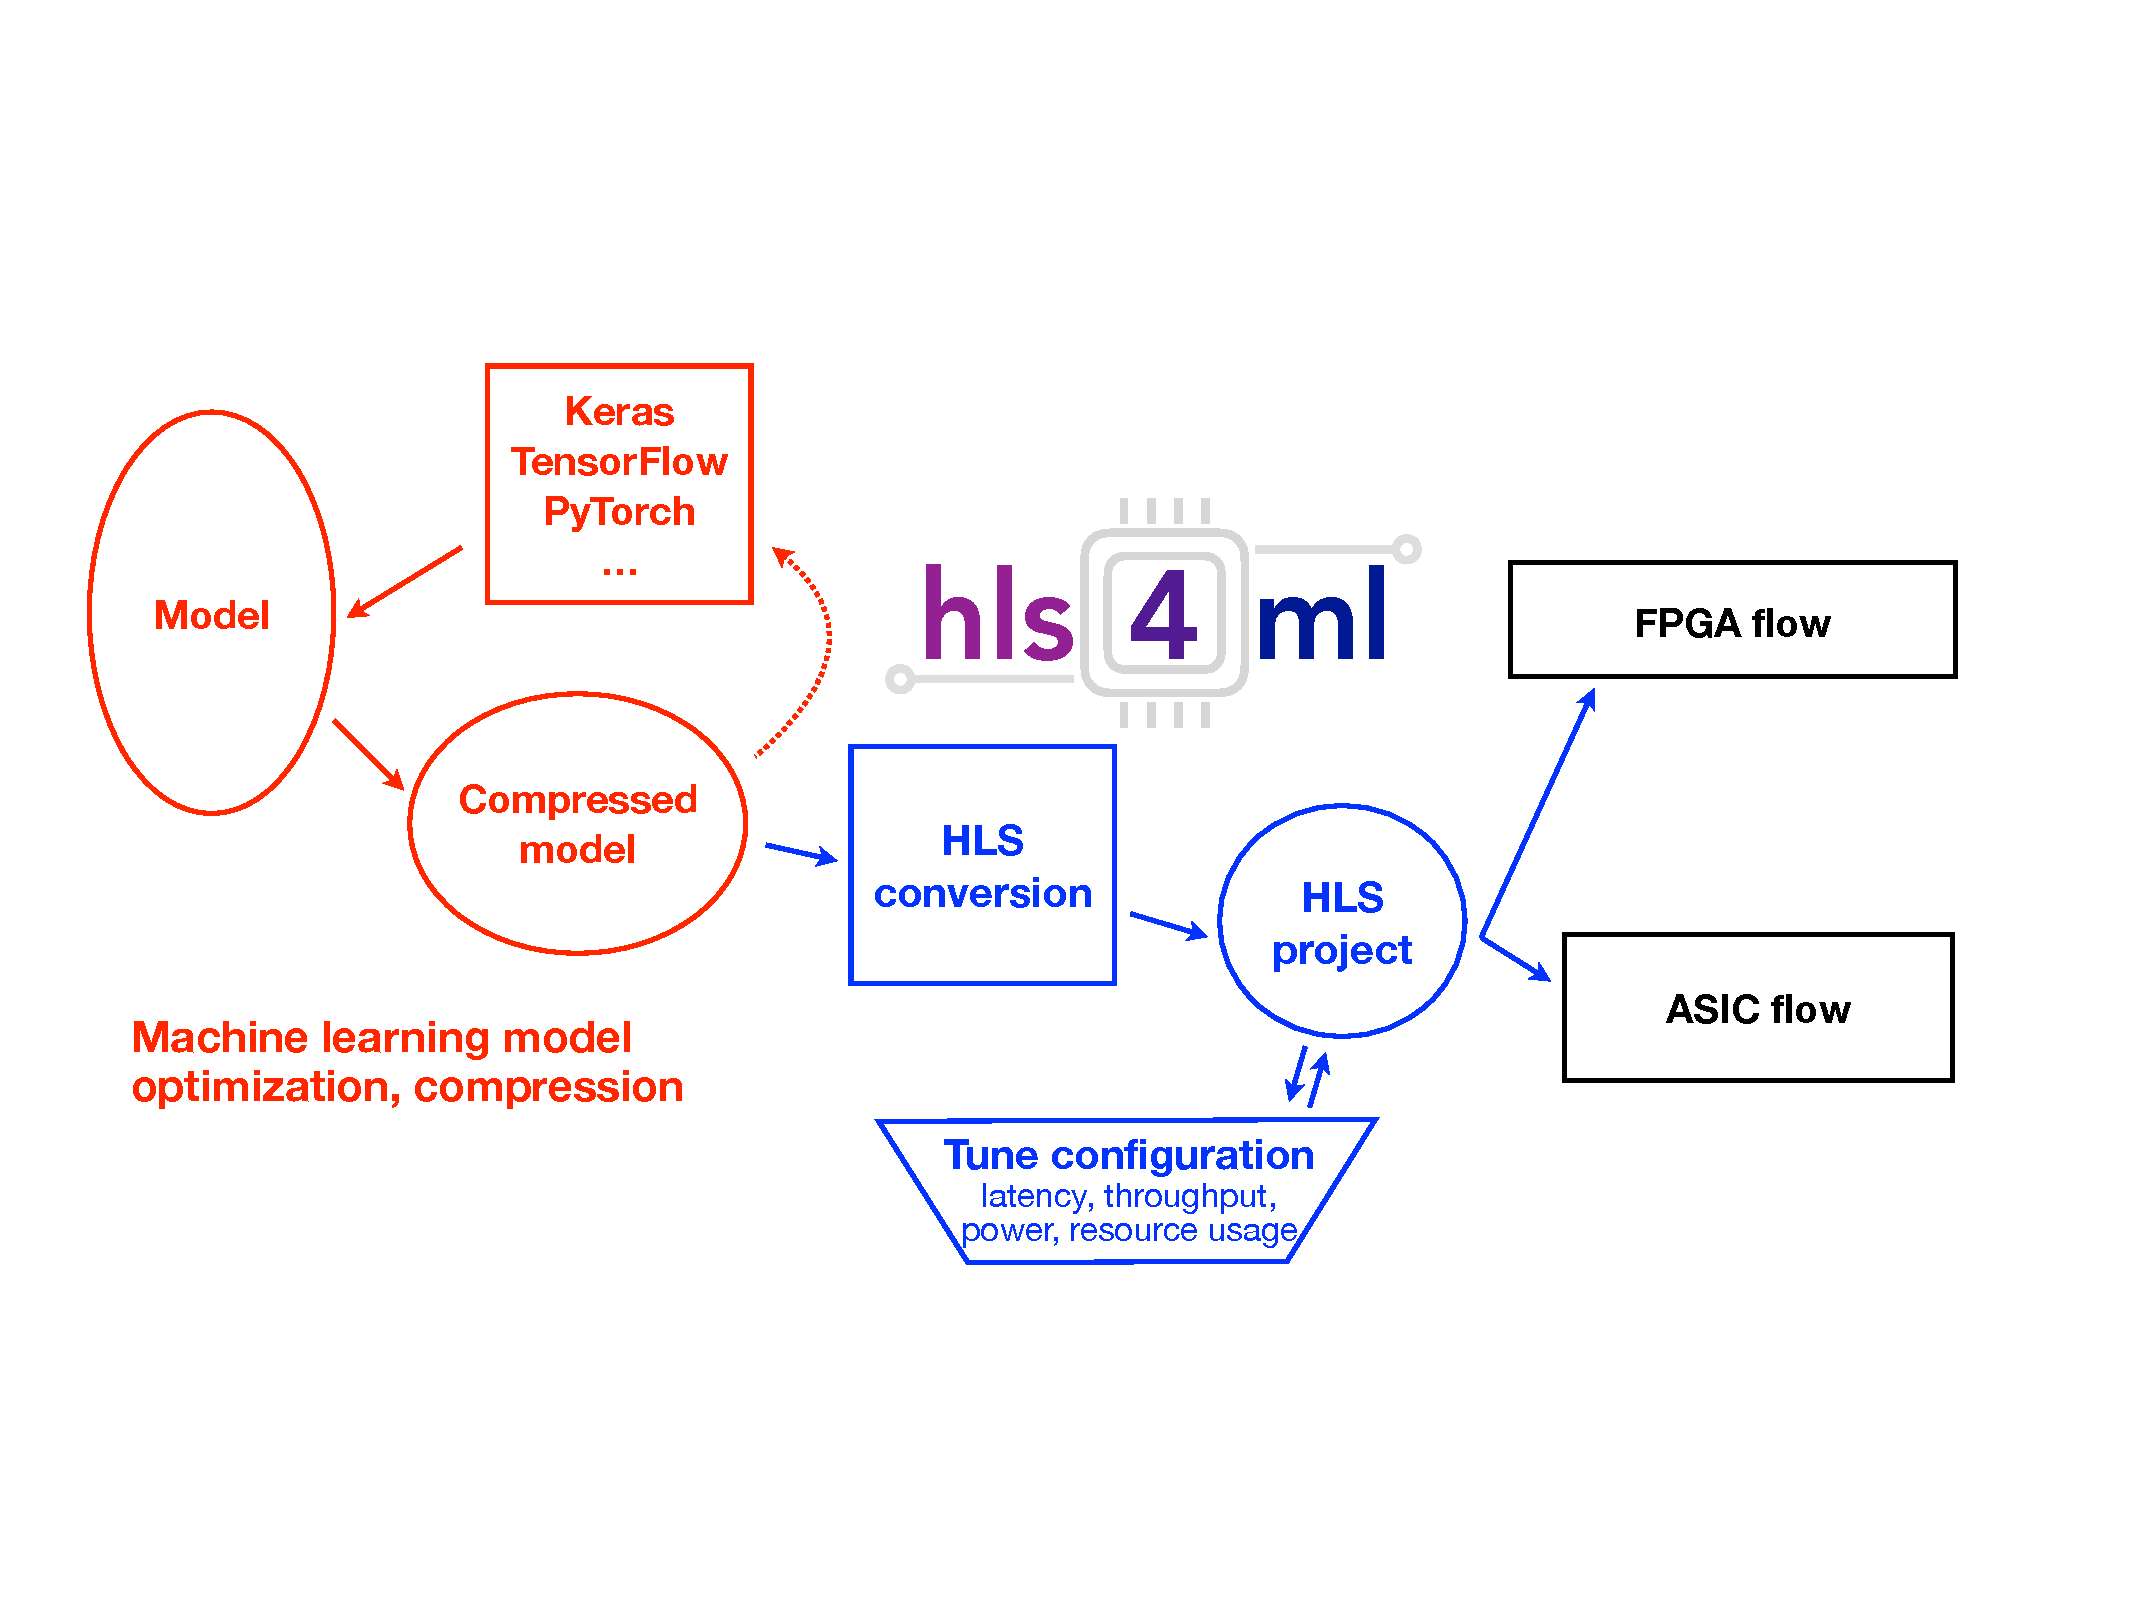
\includegraphics[width=0.8\textwidth]{figs/hls4ml-flow-4}
%        
 %       \caption[hls4ml workflow]{The workflow for converting a ML algorithm to a firmware block. The red sections represent the conventional AI development stages, the blue sections represent the conversion to HLS language and the black sections represent the output options.}\label{fig:hls4ml}
 %   \end{center}
%\end{figure}

